\documentclass[a4paper,12pt]{article}

%------------------------------------------------------------------------------------------%
% Déclaration des packages
%------------------------------------------------------------------------------------------%

\usepackage[french]{babel}
\frenchbsetup{StandardLists=true}
\usepackage{enumitem}
\usepackage[T1]{fontenc}
\usepackage{geometry} % pour gérer les dimensions des marges
\usepackage{eso-pic} % pour dessiner la marge
\usepackage{lipsum} % pour générer du contenu texte
\usepackage[cyr]{aeguill} % Police vectorielle TrueType, guillemets fran¸cais
\usepackage{epsfig} % pour g´erer les images
\usepackage{amsmath, amsthm} % tr`es bon mode math´ematique
\usepackage{amsfonts,amssymb}% permet la definition des ensembles
\usepackage{float} % pour le placement des figure
\usepackage{url} 
\usepackage[utf8]{inputenc}
\usepackage{amssymb}
\usepackage{graphicx}
\usepackage{ulem}
\usepackage{array}	
\usepackage{listings}
\usepackage{siunitx}
\usepackage{fancybox}
\usepackage{wrapfig}
\usepackage{caption}
 \usepackage{hyperref}
\usepackage{listings}
\usepackage{xcolor}
\usepackage{booktabs}
\usepackage{fancyhdr}
\usepackage{tabularx}
%\usepackage[style=authoryear,backend=biber]{biblatex}
%\addbibresource{references.bib} 

% To handle bibliography
\usepackage[backend=bibtex, style=ieee, sorting=ynt]{biblatex} %Imports biblatex package
\addbibresource{references.bib} %Import the bibliography file

\lstdefinelanguage{Dockerfile}{
  keywords={FROM, RUN, CMD, LABEL, MAINTAINER, EXPOSE, ENV, ADD, COPY, ENTRYPOINT, VOLUME, USER, WORKDIR, ARG, ONBUILD, STOPSIGNAL, HEALTHCHECK, SHELL},
  keywordstyle=\color{blue}\bfseries,
  identifierstyle=\color{black},
  sensitive=false,
  comment=[l]{\#},
  commentstyle=\color{gray}\ttfamily,
  stringstyle=\color{green},
  morestring=[b]",
  morestring=[b]',
}

\lstdefinelanguage{Python}{
  keywords={True, False, None, await, break, class, def, if, else, elif, for, while, continue, return, and, or, not, in, is, try, except, finally, raise, assert},
  keywordstyle=\color{blue}\bfseries,
  ndkeywords={import, from, as, with, print, yield},
  ndkeywordstyle=\color{darkgray}\bfseries,
  identifierstyle=\color{black},
  comment=[l]{\#},
  commentstyle=\color{green}\ttfamily,
  stringstyle=\color{green},
  morestring=[b]',
  morestring=[b]",
  sensitive=true,
}

\setlength{\parindent}{0pt}


\pagestyle{fancy}
\fancyhf{} % Efface les configurations précédentes
\fancyhead[L]{
\includegraphics[width=0.3\textwidth]{images/DS4HlogocouleurFR.png} \hfill} % Titre du rapport à gauche
\fancyhead[R]{\textit{TATIA : Classification et recommandation d'articles}} % Nom de l'auteur à droite
\fancyfoot[R]{\thepage} % Numéro de page au centre
\fancyfoot[L]{Master 1 informatique} % Numéro de page au centre

% To handle bibliography
%\usepackage[backend=bibtex, style=ieee, sorting=ynt]{biblatex} %Imports biblatex package
%\addbibresource{references.bib} %Import the bibliography file

\geometry{top=25mm, bottom=25mm, left=20mm, right=1cm}
\setlength\headheight{10mm}
\DeclareUnicodeCharacter{2212}{-}
\renewcommand{\thefootnote}{\fnsymbol{footnote}}
\renewcommand{\thefootnote}{\fnsymbol{footnote}}
\newcommand{\chatgptprompt}[1]{
    \vspace{10pt}
    \noindent\textbf{ChatGPT Prompt:}\\
    \fbox{
        \parbox{\textwidth}{
            \texttt{#1}
        }
    }
    \vspace{10pt}
}



\geometry{a4paper, margin=1in}

\title{\huge\bf  Rapport de projet Tatia}
\author{HADDOU Amine et BOULLI Marouan} 
\begin{document}

\begin{titlepage}
    \begin{center}
        
\includegraphics[width=0.3\textwidth]{./images/DS4HlogocouleurFR.png} \hfill
        
\includegraphics[width=0.10\textwidth]{./images/tampon-3IA.png} \hfill
        \textbf{
\includegraphics[width=0.3\textwidth]{images/logo_master.png}} \\
        
        \vspace{3.5cm}
        
        
        
        \textbf{\LARGE Projet TATIA}
        
        \vspace{2.5cm}
        
        \rule{\linewidth}{0.5mm} \\[0.4cm]
        {\LARGE \bfseries Classification et recommandation d'articles\\[0.5cm] }
        \rule{\linewidth}{0.5mm} \\[1.5cm]
        
        \textbf{Authors:}\\ BOULLI Marouan \& HADDOU Amine \\
        
        \vspace{0.5cm}
        
        \textbf{Mentor:} \\
        CABRIO Elena\\
       
        
    \end{center}
\end{titlepage}

\newpage
\maketitle
\tableofcontents

\newpage

\section{Contexte et objectif}


Ce projet s'inscrit dans le cadre de l'unité d'enseignement Tatia (Traitement automatique du texte en intelligence artificielle) et a pour but de mettre en application les connaissances relatives au traitement automatique du texte acquises au cours des enseignements.\\

Pour ce faire, un système de classification et de recommandation d'articles d'actualité est développé.

L'idée est la suivante : 
\begin{itemize}
    \item Un utilisateur fournit en entrée un article d'actualité non classifié.
    \item Cet article est classifié dans l'une des 5 classes présentes dans le jeu de données utilisé pour l'entraînement du modèle (\textit{buisness}, \textit{entertainment}, \textit{politics}, \textit{sport} and \textit{tech})
    \item Un algorithme calcule la similarité entre cet article et d'autres articles appartenant à la même classe contenus dans le jeu de données étiquetées.
    \item Un classement des articles en fonction de leur similarité avec l'article fournit par l'utilisateur est réalisé et l'algorithme recommande les trois articles ayant les scores de similarité les plus élevés.
\end{itemize}

\begin{figure}[h]
  \centering
  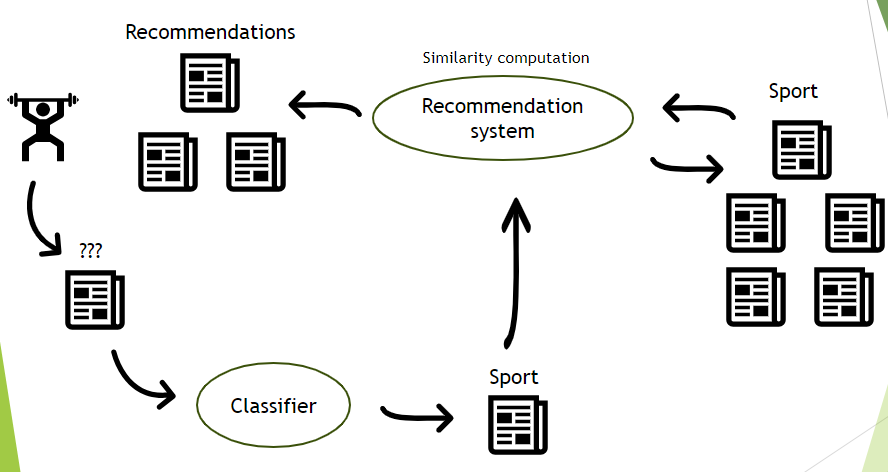
\includegraphics{./images/recommendation_system.png}
  \caption{Système de recommandation}
  \label{fig:recommendationSystem}
\end{figure}



L'article fournit par l'utilisateur est classifié avant de réaliser le calcul de similarité pour filtrer les articles sur lesquels le calcul de similarité est effectué. Ce faisant, on écarte tous les articles ne traitant pas du même thème. Le calcul de similarité n'est donc pas réalisé sur ces articles, économisant ainsi des ressources de calcul (point important si l'on considère des grandes bases de données).\\

Un des principaux challenges liés à ce projet concerne l'évaluation du système de recommandation. En effet, habituellement, l'évaluation de ce type de modèle implique la participation de plusieurs personnes chargés d'évaluer la qualité des recommandations. Toutefois, une tentative d'automatisation de cette évaluation suivant deux méthodes différentes est implémentée dans ce projet : 
\begin{itemize}
    \item Une évaluation basée sur la proportion de mots-clés communs entre l'article fournit par l'utilisateur et les articles recommandés.
    \item Une autre basée sur une comparaison avec les résultats obtenus en utilisant des LLMs (Large Language Models).
    \item Une évaluation utilisateur "manuelle" réalisée par nous-mêmes.
\end{itemize}

Ces méthodes sont présentées et discutées plus loin dans ce rapport.

\section{Données}

\subsection{Description}

Le jeu de données utilisé contient des articles d'actualité de la BBC disponible sur \href{ https://www.kaggle.com/c/learn-ai-bbc}{Kaggle} \cite{kaggle}.\\

Il est composé d'un ensemble de données d'entraînement contenant 1490 articles étiquetés suivant les catégories \textit{buisness}, \textit{entertainment}, \textit{politics}, \textit{sport} and \textit{tech}, et d'un ensemble de données de test comportant 735 articles non étiquetés. Le jeu de données de test n'est pas étiqueté car il est d'usage dans les compétitions Kaggle de garder une partie des données non étiquetée afin de s'en servir comme matériel d'évaluation des modèles des participants à la compétition.\\

Le premier ensemble de données étiquetés est utilisé pour l'entraînement et l'évaluation du modèle de classification, ainsi que pour servir de base de données d'articles étiquetés pouvant être recommandés par l'algorithme de recommandation.

Le second ensemble de données non étiquetées est quant à lui utilisé comme base de données d'articles pouvant être fournis par l'utilisateur. L'utilisateur choisit un article non étiqueté dans cette base de données, cet article est ensuite classsifié par l'algorithme de classification puis donné en entrée de l'algorithme de recommandation qui donne en sortie les trois articles les plus similaires appartenant à la même classe.\\

Il est important de vérifier que le jeu de donnée n'est pas biaisé en sur-représentant (resp. sous-représentant) une catégorie d'articles. Si c'est le cas, le modèle est susceptible de favoriser la prédiction des classes les plus représentés.

\begin{figure}[H]
  \centering
  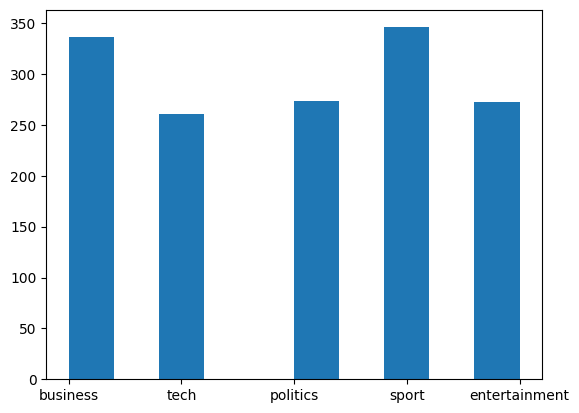
\includegraphics{./images/class_balanced.png} % Spécifiez le chemin de votre image
  \caption{Proportion des catégories d'article}
  \label{fig:classBalance}
\end{figure}

Ce jeu de données est bien équilibré avec des catégories qui représentent de $17.5 \%-23.3\%$ de l'ensemble des données (pour cinq classes, l'équilibre parfait est à 20\%). Nul besoin de sur-échantillonner ou sous-échantillonner les classes.\\

\subsection{Prétraitement}

Avant d'entamer l'implémentation de l'algorithme, il est essentiel de débuter par le prétraitement du jeu de données. Cette phase revêt une importance cruciale, car elle conditionnera la qualité de nos données et, par conséquent, celle des prédictions de notre algorithme.

L'idée est de retirer tout ce qui n'apporte pas de plus-value sémantique, pusique c'est la sémantique qui nous intéresse ici.\\

Pour ce faire, trois traitements sont réalisés : 
\begin{itemize}
    \item \textbf{Supprimer les éléments de ponctuation}.
    \item \textbf{Retirer les mots à faible valeur sémantique (stop words)} : mots grammaticaux, mots de liaison, etc.
    \item \textbf{Appliquer la lemmatisation} : uniformiser les mots pour faciliter l'apprentissage du modèle. Le WordNetLemmatizer de la bibliothèque \textit{nltk} \cite{nltk} est utilisé.
\end{itemize}

Voici un exemple d'extrait d'article avant et après prétraitement :\\

\textbf{Avant prétraitement}\\

\textit{worldcom ex-boss launches defence lawyers defending former worldcom chief bernie ebbers against a battery of fraud charges have called a company whistleblower as their first witness.  cynthia cooper  worldcom s ex-head of internal accounting  alerted directors to irregular accounting practices at the us telecoms giant in 2002. [...]}\\

\textbf{Après prétraitement}\\

\textit{worldcom exboss launch defence lawyer defending former worldcom chief bernie ebbers battery fraud charge called company whistleblower first witness cynthia cooper worldcom exhead internal accounting alerted director irregular accounting practice u telecom giant 2002 [...]}\\

\subsection{Vectorisation}

Une fois prétraitées, les données textuelles doivent être transformées en données numériques afin que le modèle puisse effectuer des calculs et des prédictions sur ces données.\\

Pour ce faire, différentes techniques de vectorisation peuvent être utilisées. Dans le cadre de ce projet, deux techniques sont utilisées : 
\begin{itemize}
    \item \textbf{TF-IDF} (Term Frequency Inverse Document Frequency)
    \item \textbf{Doc2Vec}
\end{itemize}

\subsubsection{TF-IDF}

Le TF-IDF, qui signifie "Term Frequency-Inverse Document Frequency" (Fréquence du Terme - Fréquence Inverse du Document), est une mesure statistique utilisée pour évaluer l'importance d'un mot dans un document, qui fait partie d'une collection ou d'un corpus de plusieurs documents.\\

La \textbf{Fréquence du Terme} (TF), mesure la fréquence d'un mot dans un document donné. Cela signifie simplement combien de fois un mot apparaît dans le document. Plus un mot est fréquent dans un document, plus sa valeur de TF est élevée. Cependant, cette mesure ne prend pas en compte le fait que certains mots peuvent être fréquents dans tous les documents en général.\\

La \textbf{Fréquence Inverse du Document} (IDF) mesure à quel point un mot est commun ou rare dans l'ensemble du corpus. IDF donne plus de poids aux mots qui sont rares dans le corpus entier, et moins de poids aux mots qui sont communs. Cela aide à distinguer les mots qui sont vraiment significatifs pour un document particulier.\\

En combinant ces deux mesures, TF-IDF permet de représenter les documents de manière numérique en attribuant à chaque mot un score qui reflète à la fois sa fréquence dans un document particulier et son importance dans l'ensemble du corpus. Les mots avec des scores TF-IDF élevés sont considérés comme plus importants, et ceux avec des scores bas sont moins significatifs.\\

Ci-dessous les formules permettant de calculer le TF-IDF.\\

$\text{TF}(t, d) = \frac{\text{Nombre de fois que le terme } t \text{ apparaît dans le document } d}{\text{Nombre total de termes dans le document } d}$\\

$\text{IDF}(t, D) = \log \left(\frac{\text{Nombre total de documents dans le corpus } D}{\text{Nombre de documents contenant le terme } t}\right)$\\

$\text{TF-IDF}(t, d, D) = \text{TF}(t, d) \times \text{IDF}(t, D)$\\

Cette technique est implémentée dans ce projet à l'aide du \textit{CountVectorizer} et du \textit{TFIDFTransformer} de la bibliothèque \textit{scikit-learn} \cite{tfidfsklearn}.


\subsubsection{Doc2Vec}

Doc2Vec est une extension de l'approche Word2Vec pour la représentation de documents entiers. Développée par Le et Mikolov en 2014, cette méthode permet de générer une représentation vectorielle fixe pour des séquences de mots de longueur variable, comme des phrases, des paragraphes ou des documents entiers.\\

Alors que Word2Vec génère des représentations vectorielles pour des mots individuels, Doc2Vec étend ce concept en incorporant un vecteur 'document' supplémentaire pour représenter l'ensemble du document.

Pendant l'entraînement, Doc2Vec apprend simultanément les représentations vectorielles des mots et des documents en ajustant les vecteurs pour prédire les mots dans le contexte.\\

Cette technique de vectorisation présente un certain nombre d'avantages : 
\begin{itemize}
    \item \textbf{Représentation dense} : contrairement aux modèles TF-IDF qui génèrent des vecteurs de haute dimension et creux (beaucoup de zéros dans le vecteur), Doc2Vec produit des vecteurs denses, ce qui peut améliorer l'efficacité et la performance des modèles de classification.
    \item \textbf{Capture du contexte} : Doc2Vec prend en compte l'ordre des mots et le contexte, permettant de capturer des nuances sémantiques plus riches qu'une simple analyse de fréquence des mots.
    \item \textbf{Capacité à gérer des documents de tailles variables} : Doc2Vec peut traiter efficacement des documents de différentes longueurs, ce qui est particulièrement utile pour les ensembles de données hétérogènes.
\end{itemize}

C'est l'implémentation de la bibliothèque \textit{Gensim} \cite{gensim} qui est utilisée dans ce projet.



\section{Modèles de classification}

La première étape du système de recommandation consiste à classifier l'article fournit par l'utilisateur. \\

Afin d'optimiser l'efficacité de cette classification, deux modèles de classification (SVM et KNN) sont évalués et comparés utilisant les deux méthodes de vectorisation présentées précédemment. Cela donne quatre modalités d'entraînement : 
\begin{itemize}
    \item SVM + TF-IDF
    \item SVM + Doc2Vec
    \item KNN + TF-IDF
    \item KNN + Doc2Vec
\end{itemize}

Pour ces entraînements, le jeu de données étiquetées est séparé en deux parties : $77\%$ pour l'entrainement et le reste pour l'évaluation.\\

\subsection{Support Vector Machine (SVM)}

Le premier modèle choisi est le SVM. Ce modèle est très efficace pour les tailles d'ensemble de données modérées.

Il consiste à trouver un hyperplan dans un espace de caractéristiques multidimensionnel qui sépare de manière optimale les différentes classes de données (catégories d'articles).\\

L'implémentation SVM utilisée est celle de \textit{scikit-learn} \cite{svm}.\\



\subsubsection{Entraînement}

L'entraînement est réalisé avec les hyper-paramètres par défaut.\\

Un pipeline permettant d'automatiser une séries de tâches (vectorisation + entraînement + prédiction) et faciliter la réutilisation du modèle une fois exporté est créé. 

Se référer à la page \href{https://scikit-learn.org/stable/modules/compose.html}{\textit{Pipelines and composite estimators}} de la documentation scikit-learn pour plus d'informations sur les pipelines.\\

Le modèle est entraîné selon deux modalités de vectorisation : 
\begin{itemize}
    \item TF-IDF
    \item Doc2Vec
\end{itemize}

\subsubsection{Evaluation}

Ci-dessous les rapports de classification pour chacune des modalités de vectorisation.\\

\textbf{TF-IDF}\\

\begin{figure}[H]
  \centering
  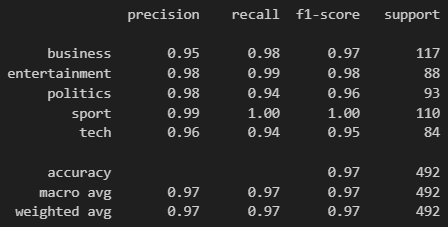
\includegraphics{images/svc_tfidf.png} 
  \caption{SVC - TFIDF Classification report}
  \label{fig:svctfidf}
\end{figure}

\textbf{Doc2Vec}\\

\begin{figure}[H]
  \centering
  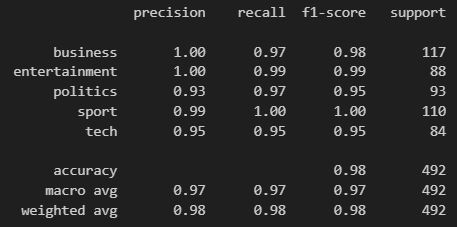
\includegraphics{images/svc_doc2vec.png} 
  \caption{SVC - Doc2Vec Classification report}
  \label{fig:svcdoc2vec}
\end{figure}

\textbf{Observations} :
\begin{itemize}
    \item Quelle que soit la modalité de vectorisation, toutes les métriques sont très bonnes.
    \item L'utilisation de Doc2Vec comme technique de vectorisation améliore légèrement les résultats du modèle (1\% en plus sur l'accuracy) ; ce qui est attendu puisque cette méthode de vectorisation est censée mieux tenir compte du contexte des mots.
\end{itemize}

\subsection{K plus proches voisins (KNN)}

Le second modèle testé est le KNN (K nearest Neighbors).\\

KNN classe un document en se basant sur les classes des K documents les plus proches (voisins) dans l'espace des caractéristiques (vecteurs).

La classe d'un nouveau document est déterminée par un vote majoritaire parmi ses K voisins. Si K = 3, par exemple, et que deux des trois voisins les plus proches appartiennent à la classe A et un à la classe B, le document sera classé en A.\\

\subsubsection{Entraînement}

La configuration d'entraînement est la même que celle utilisée pour le modèle SVM.

\subsubsection{Evaluation}

Voici les rapports de classification pour le modèle KNN suivant les deux modalités de vectorisation.\\

\textbf{TFIDF}\\

\begin{figure}[H]
  \centering
  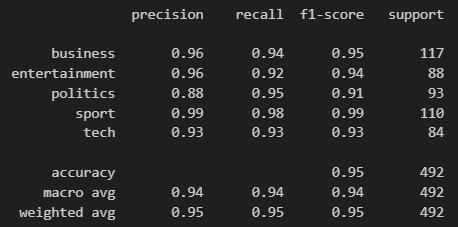
\includegraphics{images/knn_tfidf.png} 
  \caption{KNN - TFIDF Classification report}
  \label{fig:knntfidf}
\end{figure}

\textbf{Doc2Vec}\\

\begin{figure}[H]
  \centering
  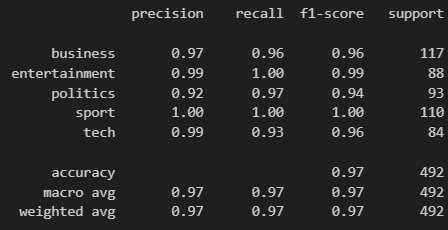
\includegraphics{images/knn_doc2vec.png} 
  \caption{KNN - Doc2Vec Classification report}
  \label{fig:knndoc2vec}
\end{figure}

\textbf{Observations} :
\begin{itemize}
    \item Comme pour le modèle SVM, les métriques sont élevées quelle que soit la modalité de vectorisation.
    \item Les résultats sont légèrement moins bons que ceux du modèle SVM (-1 / -2\%).
    \item La vectorisation avec Doc2Vec donne de meilleurs résultats ici aussi.
\end{itemize}


\section{Système de recommandation}

Une fois l'article fournit par l'utilisateur classifié, il faut calculer la similarité entre cet article et l'ensemble des articles étiquetés présents dans la base de données étiquetées. Les trois articles les plus similaires sont ensuite recommandés.\\

Cette partie vise à présenter le système de recommandation (calcul de similarité + sélection des articles à recommander) ainsi que les méthodes employées pour évaluer ce système.

\subsection{Calcul de similarité et recommandation}

La métrique utilisée pour le calcul de similarité est la \textit{similarité cosinus (cosine similarity)}.\\

La similarité cosinus est une mesure couramment utilisée pour évaluer le degré de similitude entre deux documents dans le traitement du langage naturel (NLP) et la recherche d'information. Cette mesure compare deux documents sous forme de vecteurs dans un espace multidimensionnel.

Elle est calculée comme le cosinus de l'angle entre deux vecteurs représentant deux documents. Plus la valeur est proche de 1, plus les documents comparés sont similaires.\\

Contrairement à d'autres mesures, la similarité cosinus est indépendante de la longueur des documents. Elle mesure l'orientation et non la magnitude des vecteurs, ce qui la rend utile pour comparer des documents de différentes longueurs.\\

L'implémentation utilisée dans ce projet est celle de scikit-learn \cite{cosine}.\\

Les trois articles ayant les scores de similarité cosinus les plus élevés sont recommandés. Des exemples sont présents dans le notebook de recommandation.


\subsection{Evaluation}

Trois méthodes d'évaluations du système de recommandation sont implémentées : 
\begin{itemize}
    \item Comptabilisation du nombre de mots-clés en commun entre les articles recommandés et l'article fournit par l'utilisateur.
    \item Utilisation des LLMs pour effectuer les recommandations et comparer leurs résultats avec ceux de notre système de recommandation.
    \item Evaluation manuelle basée sur notre lecture des articles.
\end{itemize}

Les deux premières ont pour objectif d'automatiser le processus d'évaluation. La dernière est la plus couramment utilisée pour les systèmes de recommandation puisque plus qualitative. 


\subsubsection{Extraction de mots-clés}

Cette méthode d'évaluation consiste à extraire k mots-clés de l'article fournit par l'utilisateur et des trois articles recommandés, en utilisant l'extracteur de mots-clés de la bibliothèque Yake \cite{yake}.\\

Un calcul de similarité est d'abord réalisé en se basant sur le nombre de mots-clés en commun. Les trois articles comportant le plus de mots-clés en commun avec l'article fournit par l'utilisateur sont recommandés.\\

Ces articles recommandés sur la base des mots-clés en commun sont ensuite comparés avec les articles recommandés obtenus avec la similarité cosinus.

Si un des articles recommandés avec la similarité cosinus est présent dans les trois articles recommandés avec l'extraction de mots-clés, on considère que la recommandation est bonne (= bonne prédiction).\\

L'opération est répétée pour chaque article du jeu de données non étiquetées (articles fournis par l'utilisateur), et une accuracy est calculée (total bonnes recommandations / total recommandation * 100).

Suivant cette méthode, on obtient une accuracy égale à 34\%.\\

\textbf{Remarque} : Cette méthode ne constitue qu'une tentative d'automatiser l'évaluation du système de recommandation. La métrique obtenue n'est pas fiable car le calcul de similarité en utilisant l'extraction de mots-clés est moins qualitatif que celui utilisant la similarité cosinus.


\subsubsection{LLMs}

L'idée ici est d'utiliser différents LLMs pour effectuer la recommandation.\\

Pour ce faire, un prompt est fournit en entrée de quatre LLMs :
\begin{itemize}
    \item OpenAI GPT4
    \item Claude AI
    \item Gemini
    \item Mistral AI
\end{itemize}

Ci-dessous le prompt en question.\\

\textit{"I'll give you one tech news article and I want you to recommend 3 articles among 10 other tech articles that I'll provide  that seem to be the most similar with the first tech article.}\\

\textit{Here's the first tech article : `article`}\\

\textit{And here are 10 tech news articles (separated with ---) from which you should recommend the 3 most similar ones with the previous article:
`articles`"}\\

L'évaluation est réalisé pour un seul article fournit en entrée et 10 articles pouvant être recommandés. Comme mentionné dans le prompt, il est demandé aux LLMs de sélectionner parmi les dix articles les trois articles les plus similaires avec celui fournit en entrée. Il s'agit ici seulement d'un test illustrant l'idée. Il faudrait répéter ce processus sur l'ensemble du jeu de données.\\

Presque tous les LLMs ont recommandé les 2 premiers articles et ont chacun proposé un article différent pour le 3ème article recommandé. Malheureusement, seul le 3ème article proposé par Gemini a été recommandé par notre algorithme.\\

Les résultats sont disponibles dans le notebook.

\subsubsection{Evaluation manuelle}

Le classement des articles par les LLMs n’a pas de grande valeur pour l'évaluation car on ne sait pas vraiment comment cette évaluation est effectuée.\\

Le meilleur moyen d’évaluer l’algorithme est de le tester manuellement avec des utilisateurs réels, qui sont finalement les mieux placés pour évaluer la qualité de la recommandation.\\

Malheureusement, nous n'avons pas pris le temps d'effectuer cette évaluation. 


\section{Conclusion}

Ce projet a permis, à travers la réalisation d'un système de recommandation d'articles, de mettre en application différents concepts et méthodes du traitement automatique du texte :
\begin{itemize}
    \item \textbf{Prétraitement des données textuelles} : pour retirer tout ce qui n'apporte pas de plus-value sémantique. cela se traduit dans ce projet par la suppression de la ponctuation et des mots à faible valeur sémantique (stop words), ainsi que par la lemmatisation.
    \item \textbf{Vectorisation} : transformer les données textuelles en données numériques pour pouvoir faire des calculs. La méthode de vectorisation Doc2Vec est plus efficace que le TF-IDF.
    \item \textbf{Modèles de classification de documents} : des modèles SVM et KNN ont été entraînés pour classifier les articles d'actualité de la BBC. Les résultats de l'évaluation ont montré l'efficacité de ces modèles et l'importance de la méthode de vectorisation utilisée.
    \item \textbf{Calcul de similarité} : en utilisant la similarité cosinus pour mesurer la proximité sémantique entre les articles.
\end{itemize}

Le point sensible réside dans l'évaluation du système de recommendation. Les tentatives d'automatisation du processus d'évaluation ne procurent pas de résultats fiables. Il semblerait que la meilleure méthode d'évaluation reste celle effectuée par les utilisateurs finaux.



\newpage

\printbibliography[
heading=bibintoc,
title={Références}
]


\end{document}